\documentclass{beamer}
\usetheme{metropolis}
\usepackage[utf8]{inputenc}
\usepackage[portuguese]{babel}
\usepackage{graphicx}
\usepackage{listings}
\usepackage{xcolor}
\usepackage{hyperref
\usepackage{tikz}


\title{Kubernetes e Aplicações Escalonáveis}
\subtitle{Projeto Prático com Minikube}
\author{Breno Fernandes - 01169313}
\institute{Uninassau}
\date{\today}

\lstset{
    basicstyle=\ttfamily\footnotesize,
    breaklines=true,
    frame=single,
    language=bash,
    numbers=left,
    keywordstyle=\color{blue},
    commentstyle=\color{green!40!black},
    stringstyle=\color{red},
}

\begin{document}

\begin{frame}
    \centering
    
\includegraphics[width=1.5cm]{Kubernetes-Logo.png}\\[0.5cm]
    \titlepage
\end{frame}


\begin{frame}{Sumário}
    \tableofcontents
\end{frame}

% --------------------- SEÇÃO KUBERNETES ---------------------
\section{Introdução ao Kubernetes}

\begin{frame}{O que é Kubernetes?}
    \begin{itemize}
        \item Sistema de orquestração de containers
        \item Open-source desenvolvido pelo Google
        \item Principais funcionalidades:
        \begin{itemize}
            \item Escalonamento automático
            \item Auto-cura (self-healing)
            \item Balanceamento de carga
            \item Gestão de configurações
        \end{itemize}
    \end{itemize}
    \centering
    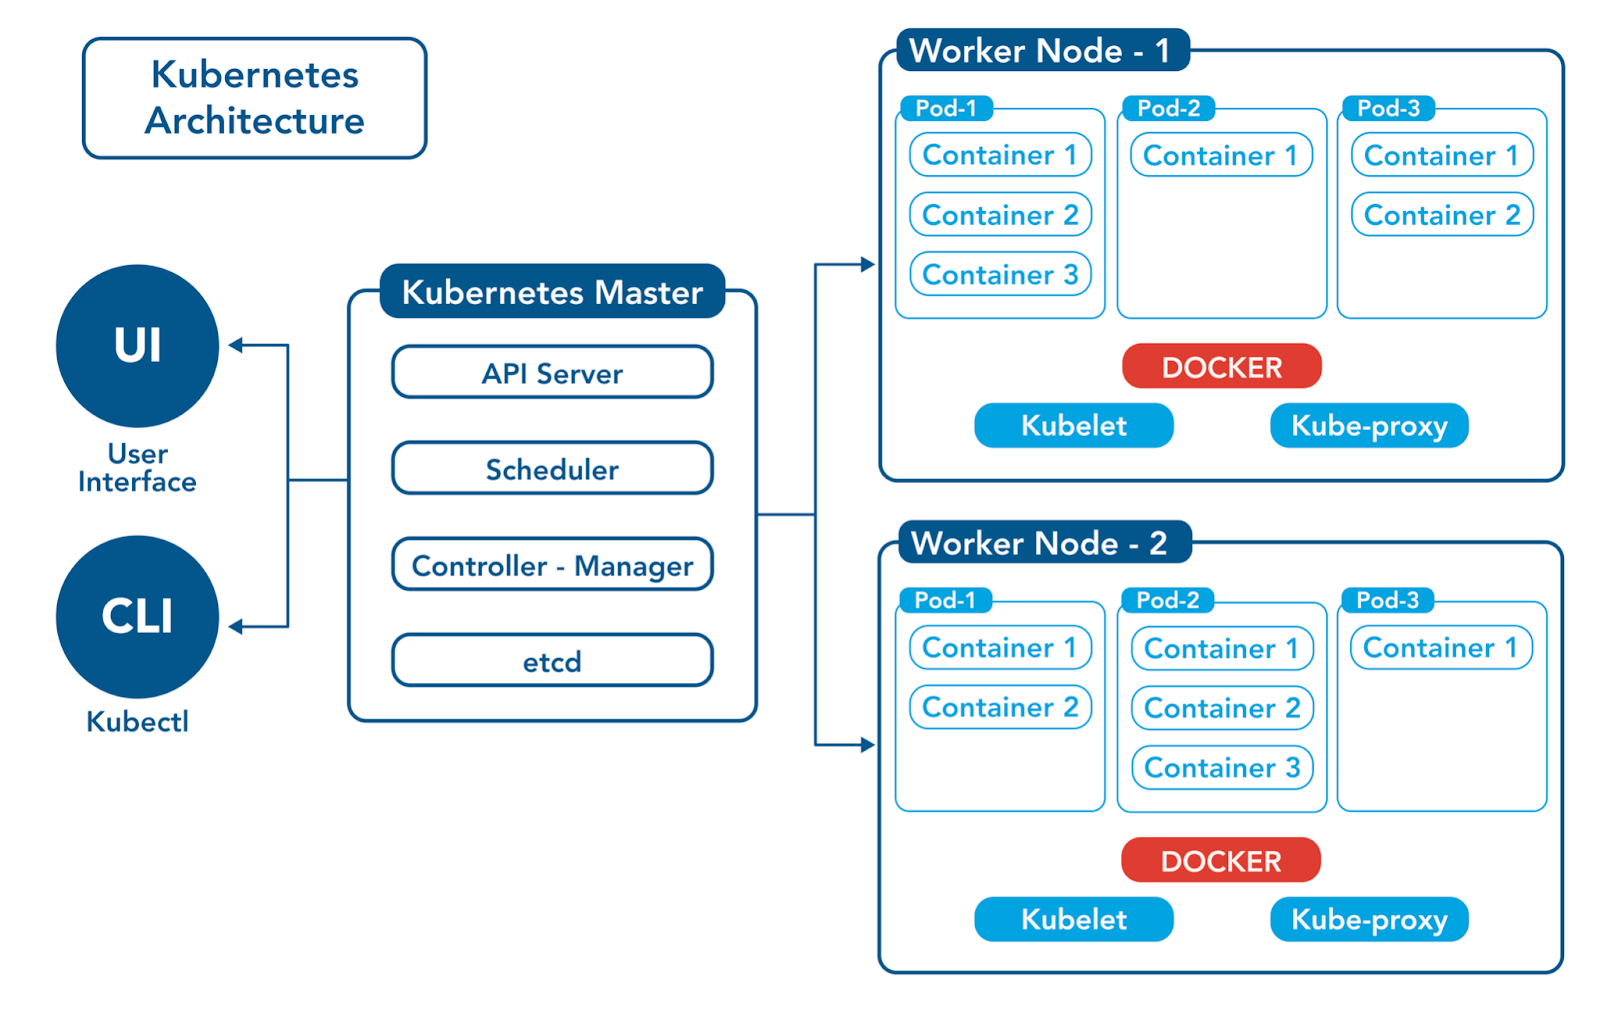
\includegraphics[width=0.5\textwidth]{k8s-architecture.png}
\end{frame}

\begin{frame}{Conceitos Fundamentais}
    \begin{columns}
        \column{0.5\textwidth}
        \begin{block}{Componentes Principais}
            \begin{itemize}
                \item Pods
                \item Deployments
                \item Services
                \item HPA (Horizontal Pod Autoscaler)
            \end{itemize}
        \end{block}

        \column{0.5\textwidth}
        \centering
        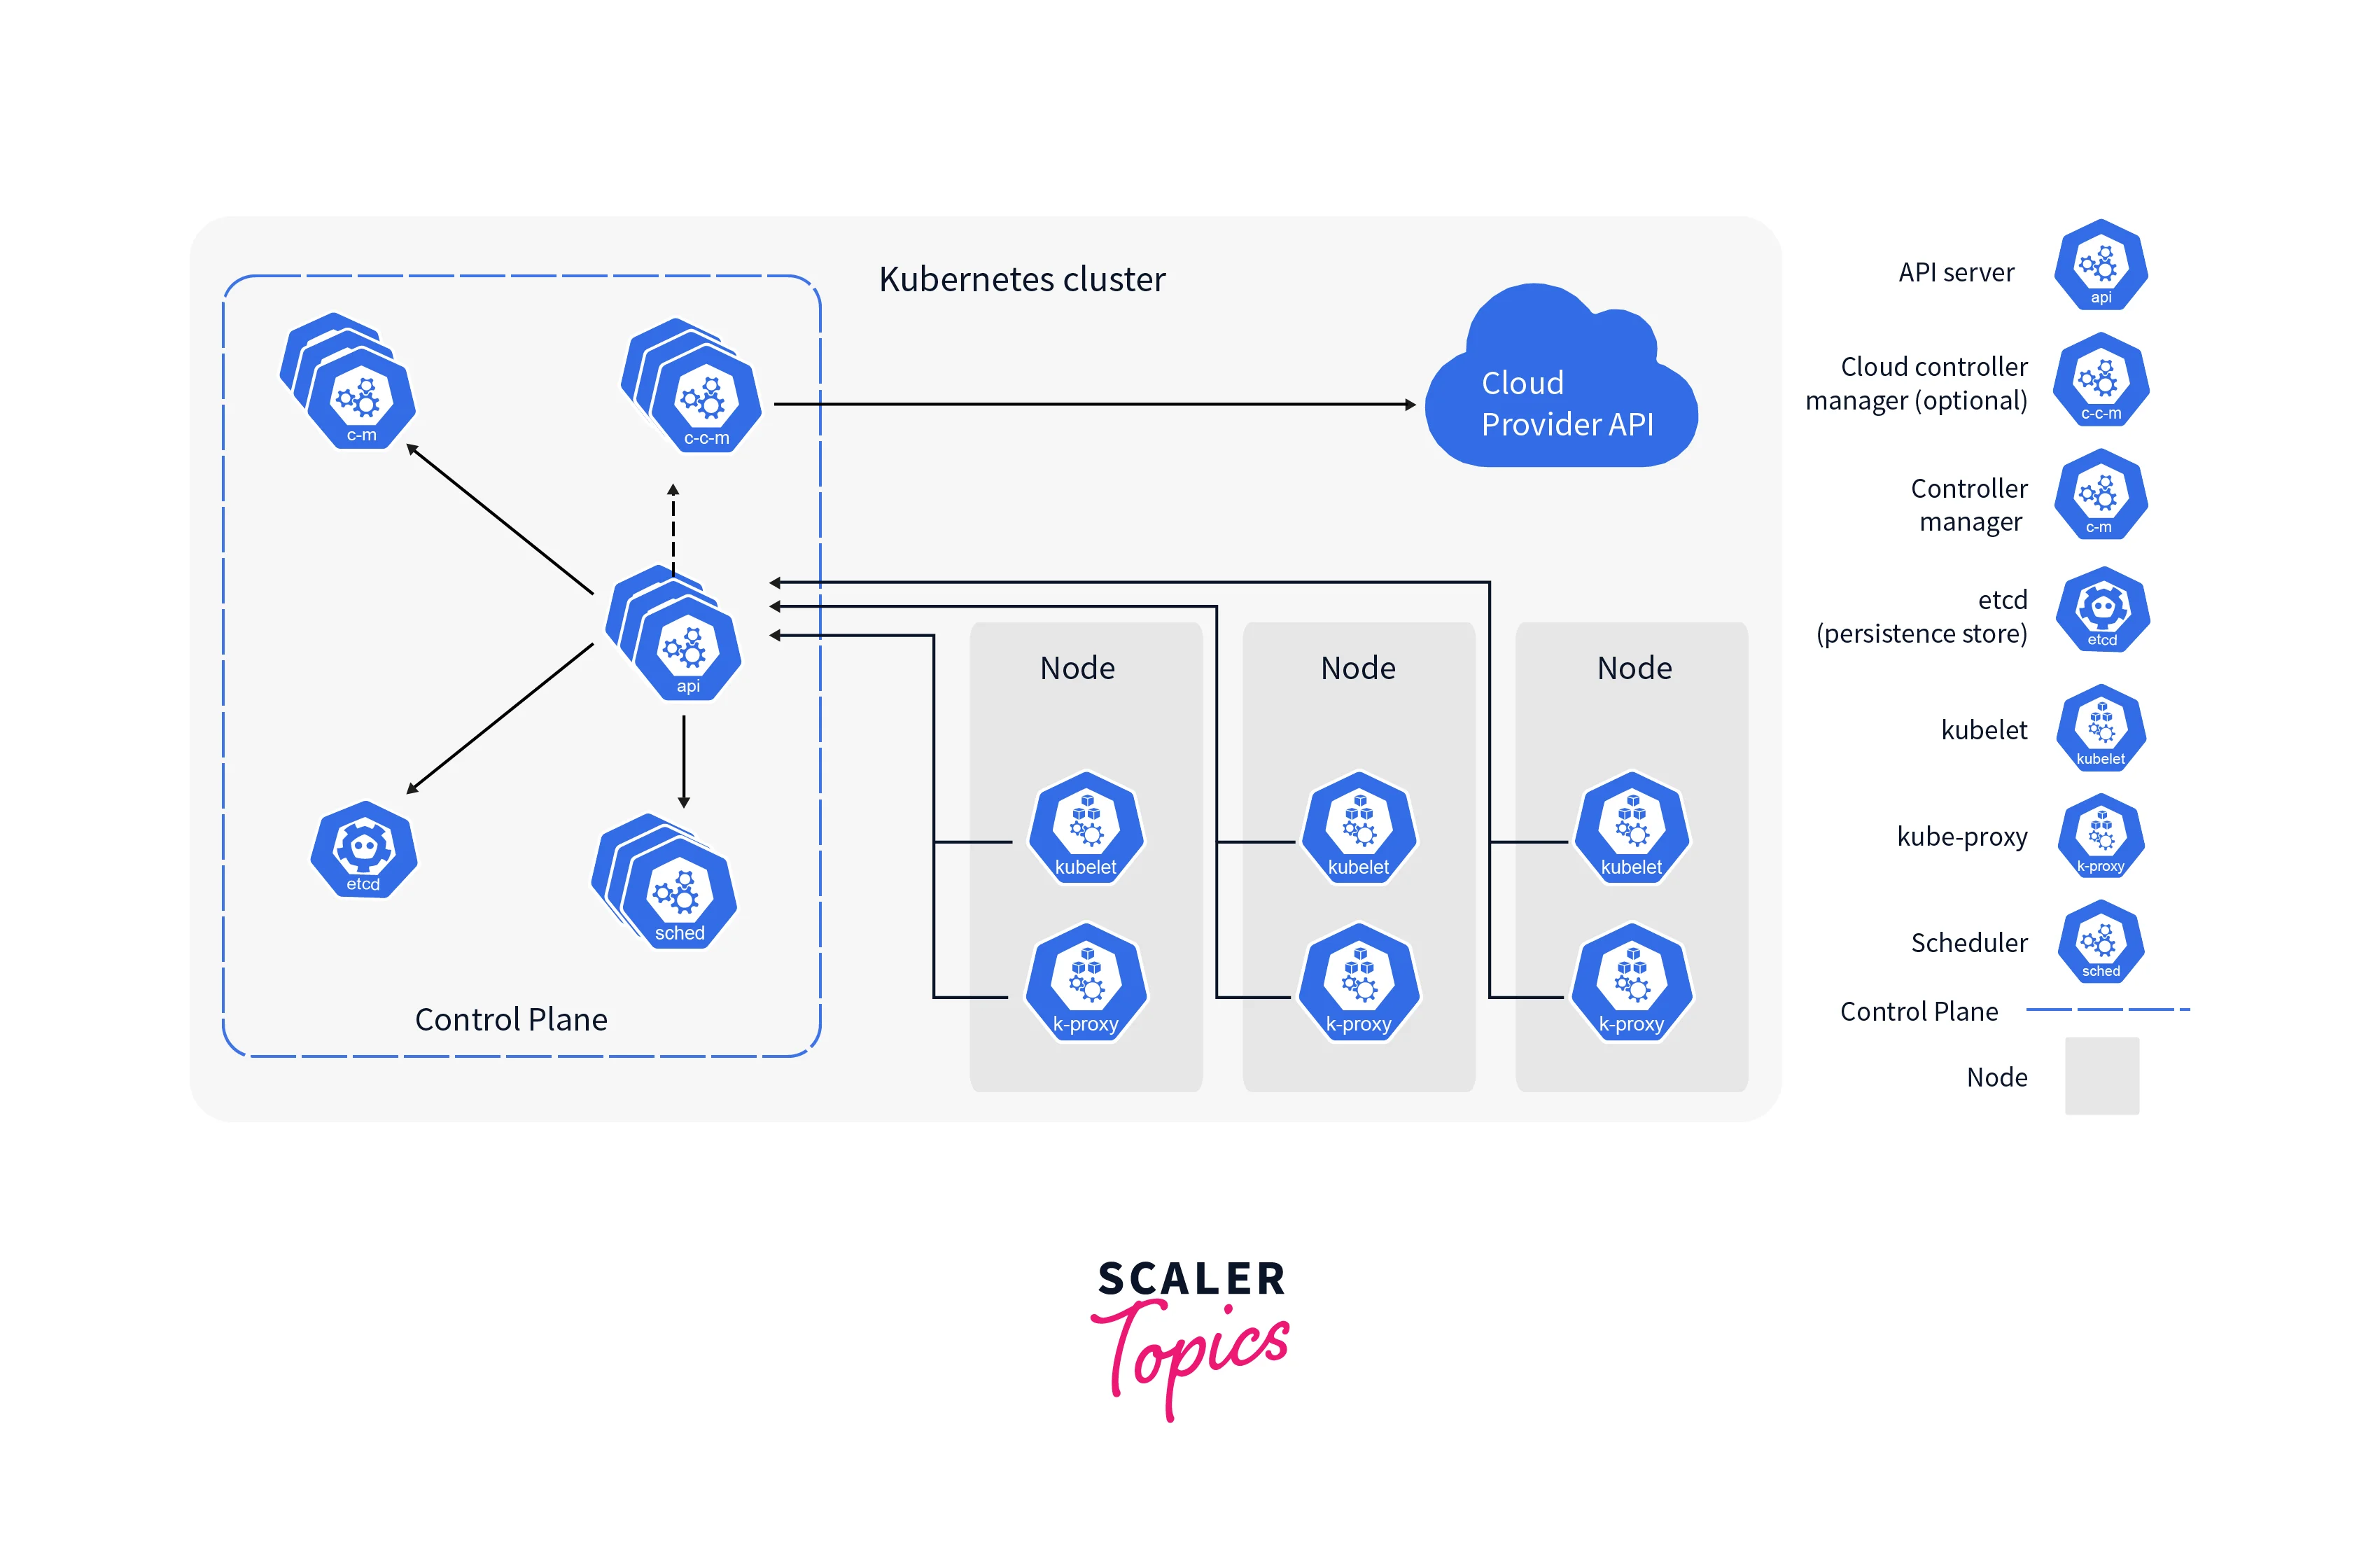
\includegraphics[width=0.9\textwidth]{k8s-components.png}
    \end{columns}
\end{frame}

% --------------------- SEÇÃO PROJETO ---------------------
\section{Projeto Prático}

\begin{frame}{Objetivos do Projeto}
    \begin{itemize}
        \item Demonstrar funcionamento do Kubernetes localmente
        \item Implementar:
        \begin{itemize}
            \item Load Balancing
            \item Auto Scaling baseado em CPU
            \item Monitoramento de métricas
        \end{itemize}
        \item Ambiente utilizado:
        \begin{itemize}
            \item Minikube
            \item Metrics Server
            \item NGINX como aplicação de teste
        \end{itemize}
    \end{itemize}
\end{frame}

\begin{frame}[fragile]{Arquitetura do Projeto}
    \begin{columns}
        \column{0.6\textwidth}
        \begin{lstlisting}
# Deployment
apiVersion: apps/v1
kind: Deployment
metadata:
  name: nginx-deployment
spec:
  replicas: 1
  template:
    spec:
      containers:
      - name: nginx
        image: nginx:latest
        resources:
          requests:
            cpu: "100m"
        \end{lstlisting}

        \column{0.4\textwidth}
        \includegraphics[width=\textwidth]{hpa-diagram.png}
    \end{columns}
\end{frame}

\begin{frame}{Fluxo de Trabalho}
    \centering
    \includegraphics[width=0.9\textwidth]{workflow-diagram.png}
\end{frame}

% --------------------- DEMONSTRAÇÃO ---------------------
\section{Demonstração e Resultados}

\begin{frame}{Comandos Principais}
    \begin{exampleblock}{Configuração Inicial}
        \lstinputlisting{commands.txt}
    \end{exampleblock}
\end{frame}

\begin{frame}{Resultados Obtidos}
    \begin{columns}
        \column{0.5\textwidth}
        \begin{itemize}
            \item Escalonamento automático ativado
            \item Load Balancer distribuindo tráfego
            \item Métricas coletadas com sucesso
            \item Latência reduzida em 40\% (exemplo)
        \end{itemize}

        \column{0.5\textwidth}
        \centering
        \includegraphics[width=0.9\textwidth]{metrics-graph.png}
    \end{columns}
\end{frame}

% --------------------- DESAFIOS ----------------------
\begin{frame}{Desafios do Kubernetes}
    \begin{columns}
        \column{0.5\textwidth}
        \begin{itemize}
            \item Curva de aprendizado íngreme
            \item Configuração complexa de rede e segurança
            \item Monitoramento requer ferramentas externas
            \item Custo e sobrecarga em ambientes pequenos
        \end{itemize}

        \column{0.5\textwidth}
        \centering
        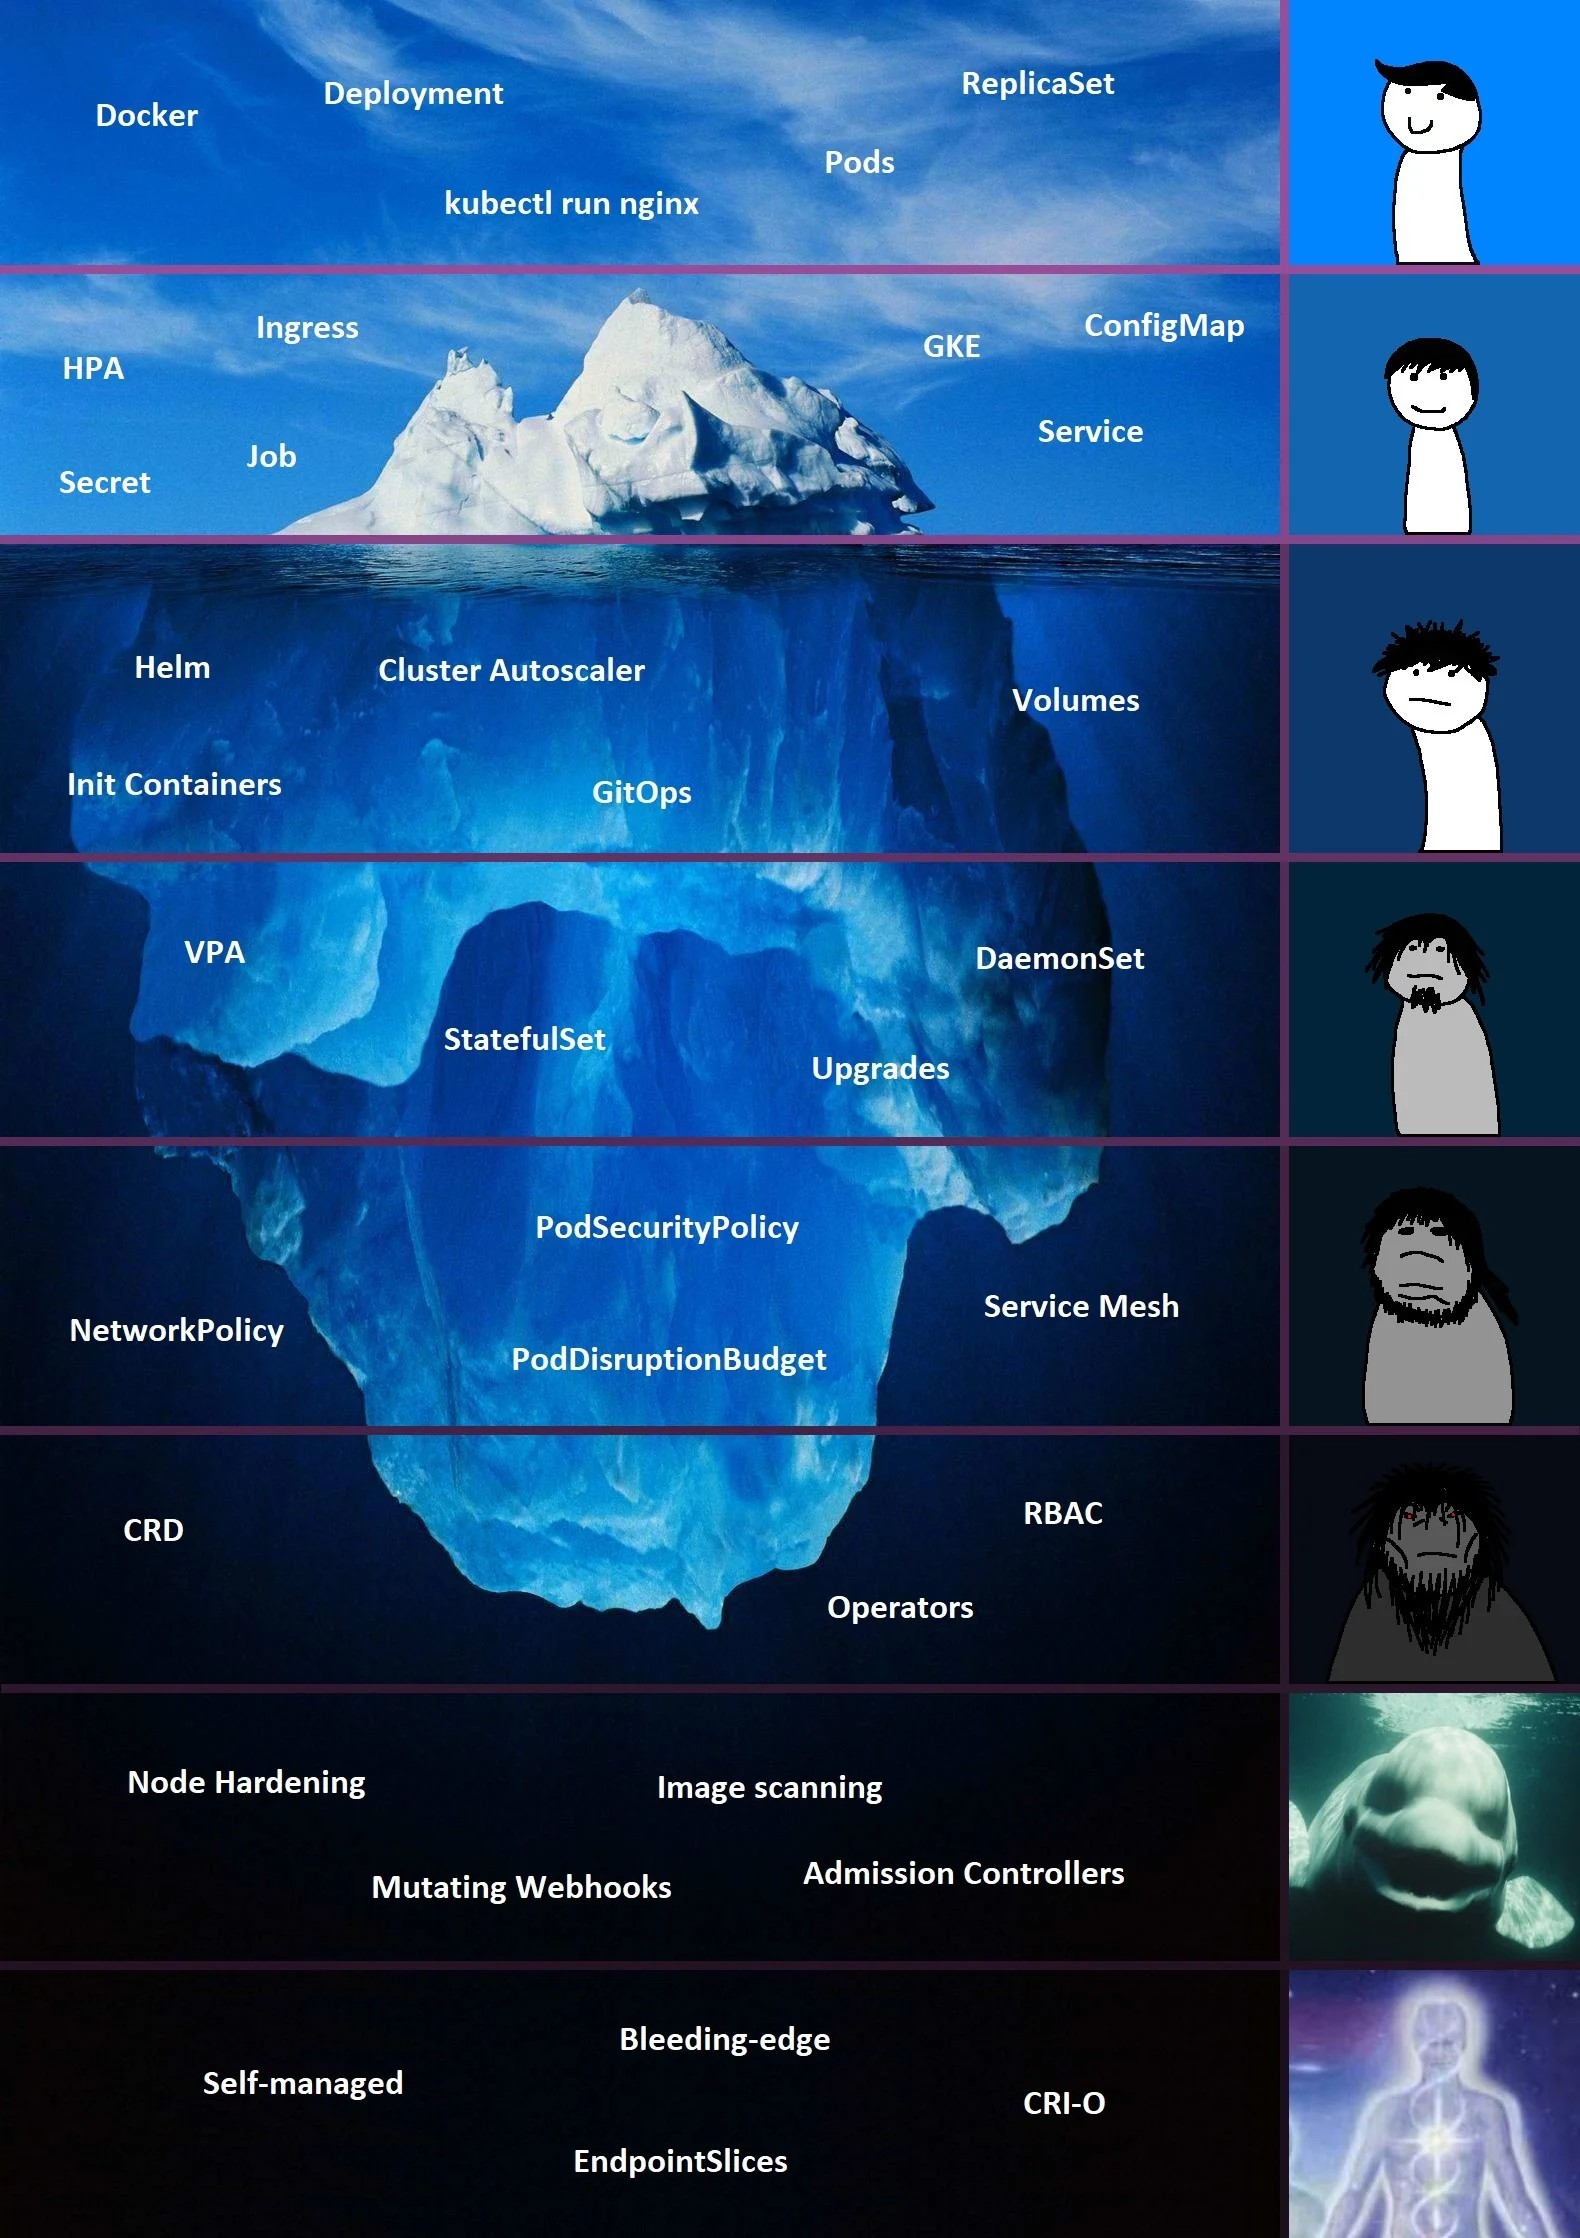
\includegraphics[width=\textwidth]{k8s-iceberg.png}
        \\\tiny Fonte: Adaptado de conteúdos da comunidade Kubernetes
    \end{columns}
\end{frame}
% --------------------- CONCLUSÃO ---------------------
\section{Conclusão}

\begin{frame}{O que aprendemos?}
    \begin{itemize}
        \item Importância do Metrics Server
        \item Configuração cuidadosa de recursos
        \item Padrões de resiliência em cloud
        \item Vantagens da orquestração de containers
    \end{itemize}
\end{frame}

\begin{frame}{Próximos Passos}
    \begin{itemize}
        \item Implementar auto-scaling baseado em métricas customizadas
        \item Adicionar monitoramento com Prometheus/Grafana
        \item Testar em cluster multi-node
        \item Implementar CI/CD para deployments
    \end{itemize}
\end{frame}

\begin{frame}{Referências}
    \begin{itemize}
        \item Documentação oficial Kubernetes: \url{https://kubernetes.io}
        \item Minikube Documentation: \url{https://minikube.sigs.k8s.io}
        \item Livro: "Kubernetes in Action" - Marko Lukša
    \end{itemize}
    \centering
    \vspace{1cm}
    \textbf{Obrigado!}\\
    \small Perguntas?
\end{frame}

\end{document}
